\documentclass[aspectratio=43,10pt]{beamer}

% ---------------------------------------------------------------- look & feel
\usetheme{Frankfurt}
\usepackage[T1]{fontenc}
\usepackage{lmodern}
\usepackage{amsmath,amssymb}
\usepackage{booktabs}
\usepackage{tikz}
\usetikzlibrary{arrows.meta,positioning,fit,calc,backgrounds}

\definecolor{tudnavy}{HTML}{0F2B46}
\definecolor{cNat}{HTML}{2A78D6}
\definecolor{cFsqF}{HTML}{EB6834}
\definecolor{cFsqJ}{HTML}{1BAF7A}
\definecolor{cJep}{HTML}{EDA100}
\definecolor{cGray}{HTML}{8A8A8A}

\setbeamercolor{structure}{fg=tudnavy}
\setbeamercolor{frametitle}{bg=tudnavy,fg=white}
\setbeamercolor{title}{bg=tudnavy,fg=white}
\setbeamercolor{section in head/foot}{bg=white,fg=tudnavy}
\setbeamercolor{subsection in head/foot}{bg=white,fg=tudnavy}
\setbeamercolor{footline}{bg=tudnavy,fg=white}
\setbeamercolor{item}{fg=tudnavy}
\setbeamercolor{block title}{bg=tudnavy,fg=white}
\setbeamercolor{block body}{bg=tudnavy!6}
\setbeamerfont{frametitle}{size=\large}
\setbeamertemplate{navigation symbols}{}
\setbeamertemplate{itemize items}[circle]
\setbeamertemplate{section in toc}[ball]
\setbeamertemplate{caption}[numbered]
\setbeamertemplate{frametitle}{%
  \nointerlineskip
  \begin{beamercolorbox}[wd=\paperwidth,ht=2.4ex,dp=1.1ex,leftskip=0.6em]{frametitle}
    \usebeamerfont{frametitle}\insertframetitle
  \end{beamercolorbox}}

% two-line footline as in the reference deck
\setbeamertemplate{footline}{%
  \leavevmode%
  \hbox{\begin{beamercolorbox}[wd=\paperwidth,ht=2.4ex,dp=0.9ex]{footline}%
    \scriptsize\hspace*{0.7em}\insertshortauthor\hfill\insertshortinstitute\hspace*{0.7em}%
  \end{beamercolorbox}}%
  \vskip0pt%
  \hbox{\begin{beamercolorbox}[wd=\paperwidth,ht=2.4ex,dp=1.1ex]{footline}%
    \scriptsize\hspace*{0.7em}\insertshorttitle\hfill\insertframenumber{} / \inserttotalframenumber\hspace*{0.7em}%
  \end{beamercolorbox}}}

% outline slide at the start of every section
\AtBeginSection[]{%
  \begin{frame}
    \vfill
    \tableofcontents[currentsection]
    \vfill
  \end{frame}}

\makeatletter\newcommand{\tabinput}[1]{\@@input #1 }\makeatother

% ---------------------------------------------------------------- title
\title[Universal Feature Extractor for Atari]{TOWARDS A UNIVERSAL FEATURE\\EXTRACTOR FOR ATARI GAMES}
\subtitle{Reconstruction, FSQ and Joint-Embedding Prediction}
\author{Sajid Ali Sadruddin}
\institute[Technische Universit\"at Dresden (TUD)]{Technische Universit\"at Dresden (TUD)}
\date{September, 2026}
\titlegraphic{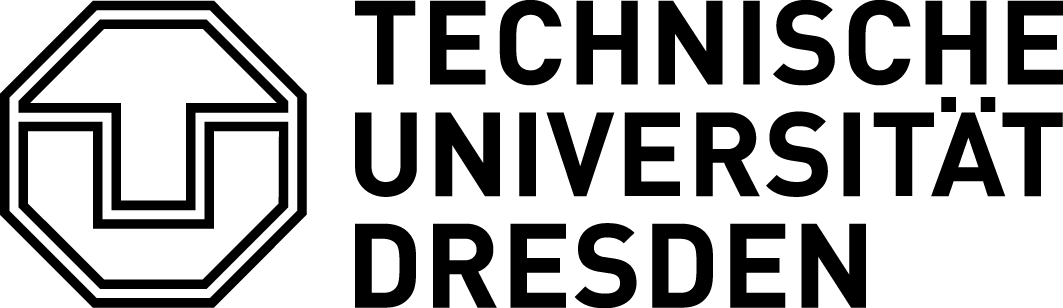
\includegraphics[width=3.2cm]{figures/tud_logo.png}}

\begin{document}

\begin{frame}
  \titlepage
\end{frame}

\begin{frame}
  \vfill
  \tableofcontents
  \vfill
\end{frame}

% =================================================================
\section{Introduction}

\begin{frame}{Introduction}
  \begin{itemize}\setlength\itemsep{0.6em}
    \item Atari games are a standard benchmark for RL from pixels
    \item Every game gives the same input: 4 stacked $84\times84$ grey-scale frames
    \item Yet each agent learns its own CNN feature extractor (NatureCNN) from scratch,
          using only the game reward
    \item The games share a lot: sprites, balls, walls, scrolling backgrounds
    \item \textbf{Idea:} pre-train \textbf{one} encoder on many games and reuse it for
          PPO on every game
  \end{itemize}
\end{frame}

\begin{frame}{Motivation and Research Questions}
  \begin{itemize}\setlength\itemsep{0.4em}
    \item A universal extractor could save interactions and compute, transfer to new games
          and give one latent space for all games
    \item Two design axes:
      \begin{itemize}
        \item \textbf{Objective:} reconstruct pixels (VQ-VAE, FSQ-VAE) or predict the next
              state in latent space (V-JEPA)
        \item \textbf{Usage:} keep the encoder \emph{frozen} or \emph{fine-tune} it with the policy
      \end{itemize}
  \end{itemize}
  \vspace{0.3em}
  \begin{block}{Research questions}
    \small
    \textbf{RQ1} Which objective gives the most useful features for PPO?\\
    \textbf{RQ2} Frozen or fine-tuned?\\
    \textbf{RQ3} Do the features generalise to unseen games?\\
    \textbf{RQ4} What does it cost, and is it interpretable?
  \end{block}
\end{frame}

% =================================================================
\section{Data \& Games}

\begin{frame}{Data Collection}
  \centering
  \resizebox{\textwidth}{!}{% Data collection and training-time processing, used as % Data collection and training-time processing, used as % Data collection and training-time processing, used as \input{figures/data_pipeline}
\resizebox{\textwidth}{!}{%
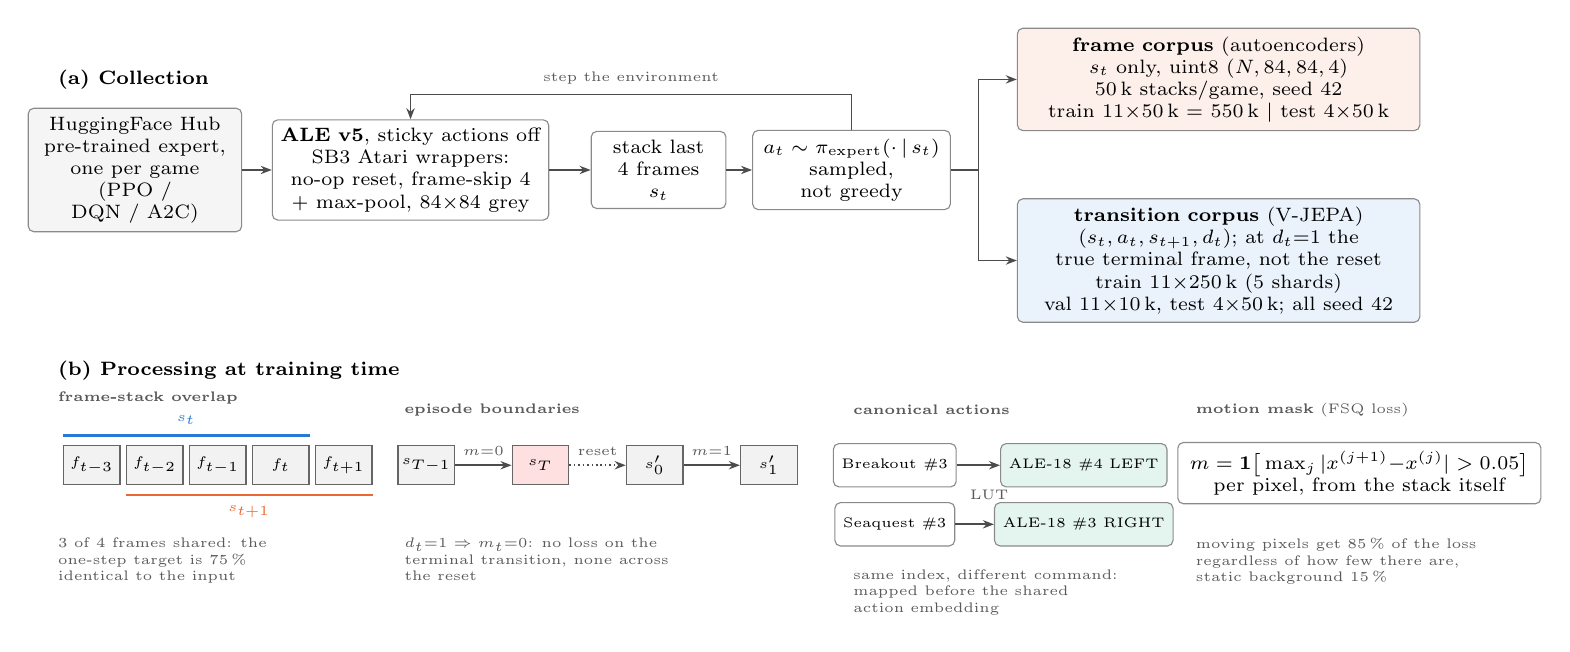
\begin{tikzpicture}[
  font=\scriptsize,
  box/.style={draw=cGray, rounded corners=2pt, align=center, inner sep=3pt, fill=white, minimum height=0.9cm},
  arr/.style={-{Stealth[length=4pt]}, draw=black!70, line width=0.6pt},
  fr/.style={draw=black!60, minimum width=0.72cm, minimum height=0.5cm, inner sep=0pt, font=\tiny},
  lab/.style={font=\tiny, text=black!65},
  ttl/.style={font=\scriptsize\bfseries, anchor=west}]

  % =========================================================== (a) collection
  \node[ttl] at (-1.1,3.35) {(a) Collection};
  \node[box, fill=gray!8, text width=2.5cm] (hub) at (0,2.2)
    {HuggingFace Hub\\pre-trained expert,\\one per game\\(PPO / DQN / A2C)};
  \node[box, text width=3.3cm] (env) at (3.5,2.2)
    {\textbf{ALE v5}, sticky actions off\\SB3 Atari wrappers: no-op reset, frame-skip 4 + max-pool, $84{\times}84$ grey};
  \node[box, text width=1.5cm] (stk) at (6.65,2.2) {stack last\\4 frames\\$s_t$};
  \node[box, text width=2.3cm] (pol) at (9.1,2.2) {$a_t\sim\pi_{\text{expert}}(\cdot\,|\,s_t)$\\sampled, not greedy};
  \draw[arr] (hub) -- (env); \draw[arr] (env) -- (stk); \draw[arr] (stk) -- (pol);
  \draw[arr] (pol.north) -- ++(0,0.45) -| node[pos=0.25, above, lab]{step the environment} (env.north);

  \node[box, fill=cFsqF!10, text width=4.9cm, anchor=west] (c1) at (11.2,3.35)
    {\textbf{frame corpus} (autoencoders)\\$s_t$ only, uint8 $(N,84,84,4)$\\50\,k stacks/game, seed 42\\train 11${\times}$50\,k = 550\,k $\mid$ test 4${\times}$50\,k};
  \node[box, fill=cNat!10, text width=4.9cm, anchor=west] (c2) at (11.2,1.05)
    {\textbf{transition corpus} (V-JEPA)\\$(s_t,a_t,s_{t+1},d_t)$; at $d_t{=}1$ the\\true terminal frame, not the reset\\train 11${\times}$250\,k (5 shards)\\val 11${\times}$10\,k, test 4${\times}$50\,k; all seed 42};
  \draw[arr] (pol.east) -- ++(0.35,0) |- (c1.west);
  \draw[arr] (pol.east) -- ++(0.35,0) |- (c2.west);

  % =========================================================== (b) processing
  \node[ttl] at (-1.1,-0.35) {(b) Processing at training time};

  % --- b1 frame overlap
  \node[lab, anchor=west] at (-1.1,-0.7) {\textbf{frame-stack overlap}};
  \foreach \i/\t in {0/$f_{t-3}$,1/$f_{t-2}$,2/$f_{t-1}$,3/$f_{t}$,4/$f_{t+1}$}
    {\node[fr, fill=gray!10] (f\i) at (-0.55+\i*0.8,-1.55) {\t};}
  \draw[cNat, line width=1pt] ([yshift=0.12cm]f0.north west) -- ([yshift=0.12cm]f3.north east)
     node[midway, above, font=\tiny, text=cNat] {$s_t$};
  \draw[cFsqF, line width=1pt] ([yshift=-0.12cm]f1.south west) -- ([yshift=-0.12cm]f4.south east)
     node[midway, below, font=\tiny, text=cFsqF] {$s_{t+1}$};
  \node[lab, align=left, anchor=north west] at (-1.1,-2.35) {3 of 4 frames shared: the\\one-step target is 75\,\%\\identical to the input};

  % --- b2 terminal mask
  \node[lab, anchor=west] at (3.3,-0.85) {\textbf{episode boundaries}};
  \node[fr, fill=gray!10] (e1) at (3.7,-1.55) {$s_{T-1}$};
  \node[fr, fill=red!12] (e2) at (5.15,-1.55) {$s_T$};
  \node[fr, fill=gray!10] (e3) at (6.6,-1.55) {$s'_0$};
  \node[fr, fill=gray!10] (e4) at (8.05,-1.55) {$s'_1$};
  \draw[arr] (e1) -- node[above, lab]{$m{=}0$} (e2);
  \draw[arr, densely dotted] (e2) -- node[above, lab]{reset} (e3);
  \draw[arr] (e3) -- node[above, lab]{$m{=}1$} (e4);
  \node[lab, align=left, anchor=north west] at (3.3,-2.35) {$d_t{=}1\Rightarrow m_t{=}0$: no loss on the\\terminal transition, none across\\the reset};

  % --- b3 action canonicalisation
  \node[lab, anchor=west] at (9.0,-0.85) {\textbf{canonical actions}};
  \node[box, minimum height=0.55cm, font=\tiny] (bk) at (9.65,-1.55) {Breakout \#3};
  \node[box, minimum height=0.55cm, font=\tiny] (sq) at (9.65,-2.3) {Seaquest \#3};
  \node[box, minimum height=0.55cm, font=\tiny, fill=cFsqJ!12] (l4) at (12.05,-1.55) {ALE-18 \#4 LEFT};
  \node[box, minimum height=0.55cm, font=\tiny, fill=cFsqJ!12] (r3) at (12.05,-2.3) {ALE-18 \#3 RIGHT};
  \draw[arr] (bk) -- (l4); \node[lab] at (10.85,-1.93) {LUT}; \draw[arr] (sq) -- (r3);
  \node[lab, align=left, anchor=north west] at (9.0,-2.75) {same index, different command:\\mapped before the shared\\action embedding};

  % --- b4 motion mask
  \node[lab, anchor=west] at (13.35,-0.85) {\textbf{motion mask} (FSQ loss)};
  \node[box, minimum height=0.55cm, text width=4.4cm, font=\scriptsize] (mm) at (15.55,-1.65)
    {\mbox{$m=\mathbf{1}\big[\max_j|x^{(j+1)}{-}x^{(j)}|>0.05\big]$}\\per pixel, from the stack itself};
  \node[lab, align=left, anchor=north west] at (13.35,-2.35) {moving pixels get 85\,\% of the loss\\regardless of how few there are,\\static background 15\,\%};
\end{tikzpicture}}

\resizebox{\textwidth}{!}{%
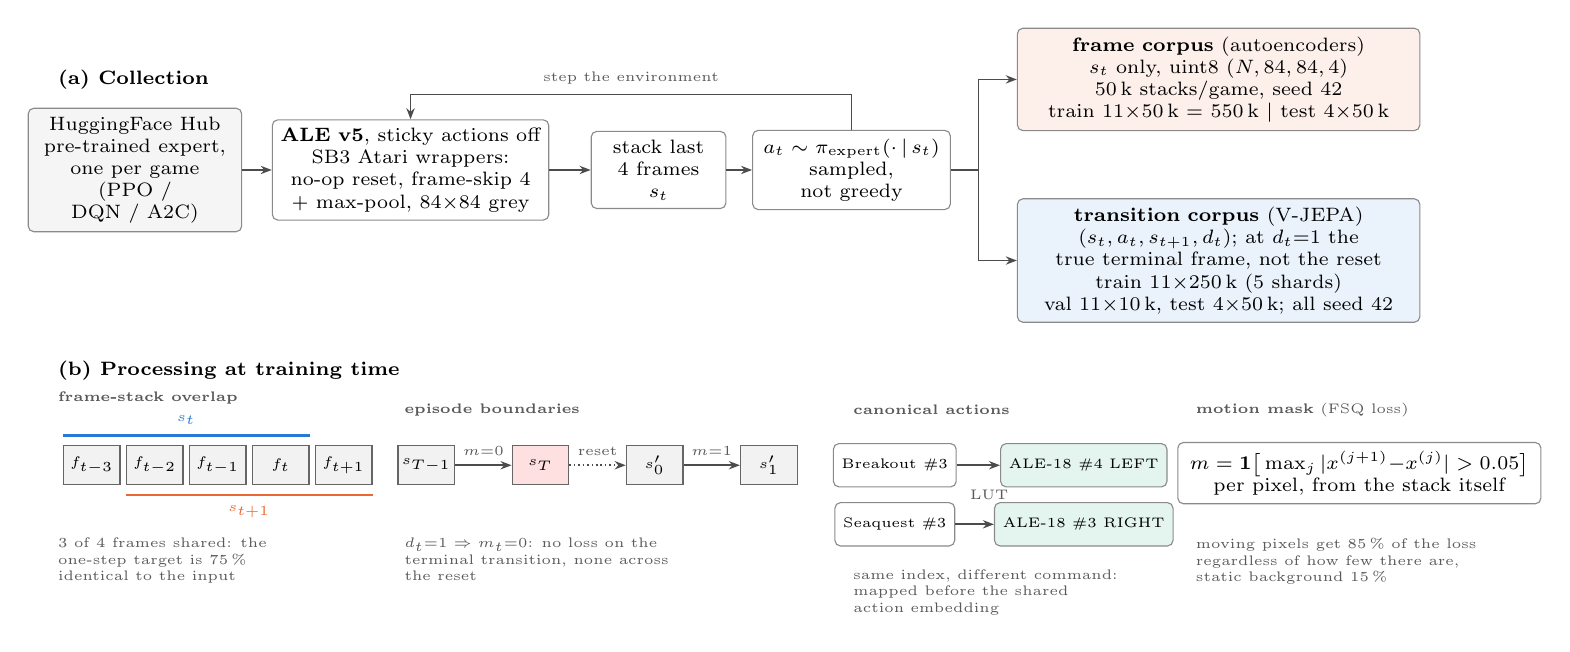
\begin{tikzpicture}[
  font=\scriptsize,
  box/.style={draw=cGray, rounded corners=2pt, align=center, inner sep=3pt, fill=white, minimum height=0.9cm},
  arr/.style={-{Stealth[length=4pt]}, draw=black!70, line width=0.6pt},
  fr/.style={draw=black!60, minimum width=0.72cm, minimum height=0.5cm, inner sep=0pt, font=\tiny},
  lab/.style={font=\tiny, text=black!65},
  ttl/.style={font=\scriptsize\bfseries, anchor=west}]

  % =========================================================== (a) collection
  \node[ttl] at (-1.1,3.35) {(a) Collection};
  \node[box, fill=gray!8, text width=2.5cm] (hub) at (0,2.2)
    {HuggingFace Hub\\pre-trained expert,\\one per game\\(PPO / DQN / A2C)};
  \node[box, text width=3.3cm] (env) at (3.5,2.2)
    {\textbf{ALE v5}, sticky actions off\\SB3 Atari wrappers: no-op reset, frame-skip 4 + max-pool, $84{\times}84$ grey};
  \node[box, text width=1.5cm] (stk) at (6.65,2.2) {stack last\\4 frames\\$s_t$};
  \node[box, text width=2.3cm] (pol) at (9.1,2.2) {$a_t\sim\pi_{\text{expert}}(\cdot\,|\,s_t)$\\sampled, not greedy};
  \draw[arr] (hub) -- (env); \draw[arr] (env) -- (stk); \draw[arr] (stk) -- (pol);
  \draw[arr] (pol.north) -- ++(0,0.45) -| node[pos=0.25, above, lab]{step the environment} (env.north);

  \node[box, fill=cFsqF!10, text width=4.9cm, anchor=west] (c1) at (11.2,3.35)
    {\textbf{frame corpus} (autoencoders)\\$s_t$ only, uint8 $(N,84,84,4)$\\50\,k stacks/game, seed 42\\train 11${\times}$50\,k = 550\,k $\mid$ test 4${\times}$50\,k};
  \node[box, fill=cNat!10, text width=4.9cm, anchor=west] (c2) at (11.2,1.05)
    {\textbf{transition corpus} (V-JEPA)\\$(s_t,a_t,s_{t+1},d_t)$; at $d_t{=}1$ the\\true terminal frame, not the reset\\train 11${\times}$250\,k (5 shards)\\val 11${\times}$10\,k, test 4${\times}$50\,k; all seed 42};
  \draw[arr] (pol.east) -- ++(0.35,0) |- (c1.west);
  \draw[arr] (pol.east) -- ++(0.35,0) |- (c2.west);

  % =========================================================== (b) processing
  \node[ttl] at (-1.1,-0.35) {(b) Processing at training time};

  % --- b1 frame overlap
  \node[lab, anchor=west] at (-1.1,-0.7) {\textbf{frame-stack overlap}};
  \foreach \i/\t in {0/$f_{t-3}$,1/$f_{t-2}$,2/$f_{t-1}$,3/$f_{t}$,4/$f_{t+1}$}
    {\node[fr, fill=gray!10] (f\i) at (-0.55+\i*0.8,-1.55) {\t};}
  \draw[cNat, line width=1pt] ([yshift=0.12cm]f0.north west) -- ([yshift=0.12cm]f3.north east)
     node[midway, above, font=\tiny, text=cNat] {$s_t$};
  \draw[cFsqF, line width=1pt] ([yshift=-0.12cm]f1.south west) -- ([yshift=-0.12cm]f4.south east)
     node[midway, below, font=\tiny, text=cFsqF] {$s_{t+1}$};
  \node[lab, align=left, anchor=north west] at (-1.1,-2.35) {3 of 4 frames shared: the\\one-step target is 75\,\%\\identical to the input};

  % --- b2 terminal mask
  \node[lab, anchor=west] at (3.3,-0.85) {\textbf{episode boundaries}};
  \node[fr, fill=gray!10] (e1) at (3.7,-1.55) {$s_{T-1}$};
  \node[fr, fill=red!12] (e2) at (5.15,-1.55) {$s_T$};
  \node[fr, fill=gray!10] (e3) at (6.6,-1.55) {$s'_0$};
  \node[fr, fill=gray!10] (e4) at (8.05,-1.55) {$s'_1$};
  \draw[arr] (e1) -- node[above, lab]{$m{=}0$} (e2);
  \draw[arr, densely dotted] (e2) -- node[above, lab]{reset} (e3);
  \draw[arr] (e3) -- node[above, lab]{$m{=}1$} (e4);
  \node[lab, align=left, anchor=north west] at (3.3,-2.35) {$d_t{=}1\Rightarrow m_t{=}0$: no loss on the\\terminal transition, none across\\the reset};

  % --- b3 action canonicalisation
  \node[lab, anchor=west] at (9.0,-0.85) {\textbf{canonical actions}};
  \node[box, minimum height=0.55cm, font=\tiny] (bk) at (9.65,-1.55) {Breakout \#3};
  \node[box, minimum height=0.55cm, font=\tiny] (sq) at (9.65,-2.3) {Seaquest \#3};
  \node[box, minimum height=0.55cm, font=\tiny, fill=cFsqJ!12] (l4) at (12.05,-1.55) {ALE-18 \#4 LEFT};
  \node[box, minimum height=0.55cm, font=\tiny, fill=cFsqJ!12] (r3) at (12.05,-2.3) {ALE-18 \#3 RIGHT};
  \draw[arr] (bk) -- (l4); \node[lab] at (10.85,-1.93) {LUT}; \draw[arr] (sq) -- (r3);
  \node[lab, align=left, anchor=north west] at (9.0,-2.75) {same index, different command:\\mapped before the shared\\action embedding};

  % --- b4 motion mask
  \node[lab, anchor=west] at (13.35,-0.85) {\textbf{motion mask} (FSQ loss)};
  \node[box, minimum height=0.55cm, text width=4.4cm, font=\scriptsize] (mm) at (15.55,-1.65)
    {\mbox{$m=\mathbf{1}\big[\max_j|x^{(j+1)}{-}x^{(j)}|>0.05\big]$}\\per pixel, from the stack itself};
  \node[lab, align=left, anchor=north west] at (13.35,-2.35) {moving pixels get 85\,\% of the loss\\regardless of how few there are,\\static background 15\,\%};
\end{tikzpicture}}

\resizebox{\textwidth}{!}{%
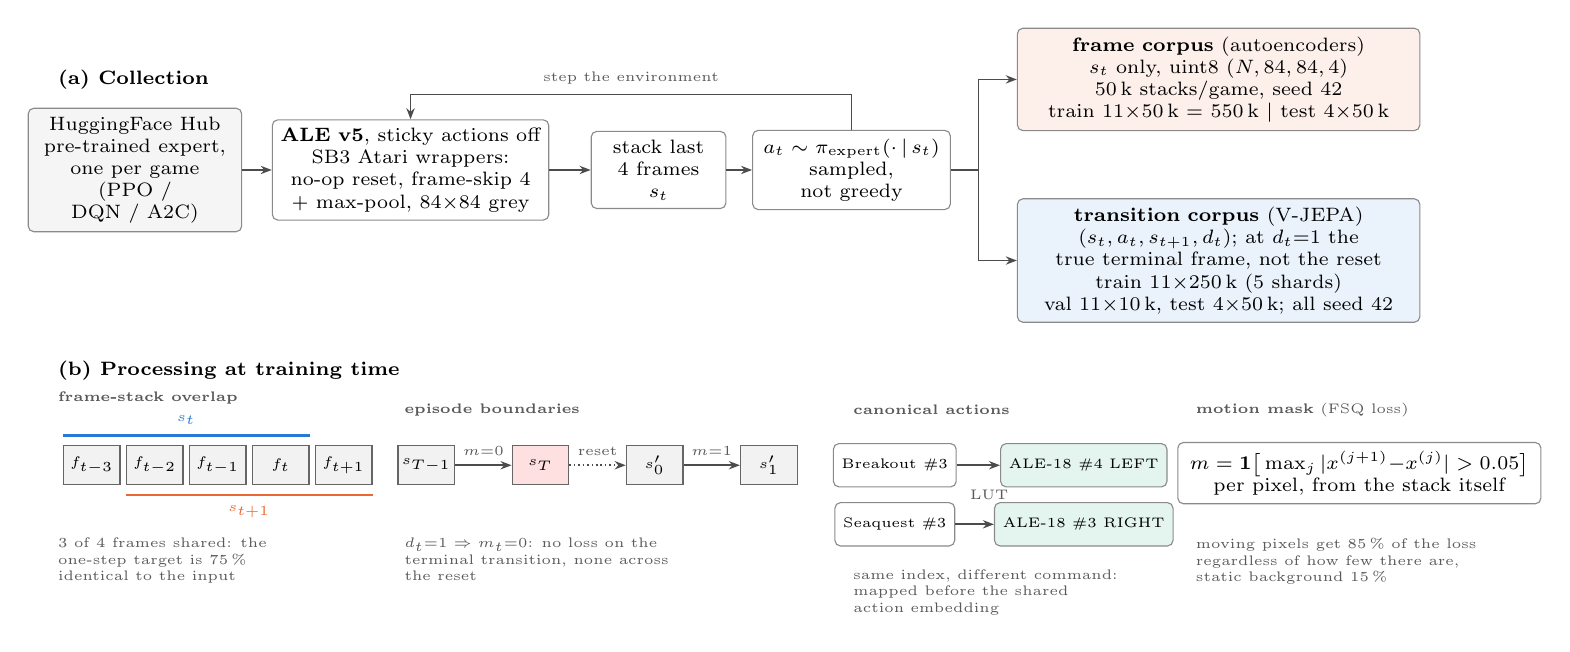
\begin{tikzpicture}[
  font=\scriptsize,
  box/.style={draw=cGray, rounded corners=2pt, align=center, inner sep=3pt, fill=white, minimum height=0.9cm},
  arr/.style={-{Stealth[length=4pt]}, draw=black!70, line width=0.6pt},
  fr/.style={draw=black!60, minimum width=0.72cm, minimum height=0.5cm, inner sep=0pt, font=\tiny},
  lab/.style={font=\tiny, text=black!65},
  ttl/.style={font=\scriptsize\bfseries, anchor=west}]

  % =========================================================== (a) collection
  \node[ttl] at (-1.1,3.35) {(a) Collection};
  \node[box, fill=gray!8, text width=2.5cm] (hub) at (0,2.2)
    {HuggingFace Hub\\pre-trained expert,\\one per game\\(PPO / DQN / A2C)};
  \node[box, text width=3.3cm] (env) at (3.5,2.2)
    {\textbf{ALE v5}, sticky actions off\\SB3 Atari wrappers: no-op reset, frame-skip 4 + max-pool, $84{\times}84$ grey};
  \node[box, text width=1.5cm] (stk) at (6.65,2.2) {stack last\\4 frames\\$s_t$};
  \node[box, text width=2.3cm] (pol) at (9.1,2.2) {$a_t\sim\pi_{\text{expert}}(\cdot\,|\,s_t)$\\sampled, not greedy};
  \draw[arr] (hub) -- (env); \draw[arr] (env) -- (stk); \draw[arr] (stk) -- (pol);
  \draw[arr] (pol.north) -- ++(0,0.45) -| node[pos=0.25, above, lab]{step the environment} (env.north);

  \node[box, fill=cFsqF!10, text width=4.9cm, anchor=west] (c1) at (11.2,3.35)
    {\textbf{frame corpus} (autoencoders)\\$s_t$ only, uint8 $(N,84,84,4)$\\50\,k stacks/game, seed 42\\train 11${\times}$50\,k = 550\,k $\mid$ test 4${\times}$50\,k};
  \node[box, fill=cNat!10, text width=4.9cm, anchor=west] (c2) at (11.2,1.05)
    {\textbf{transition corpus} (V-JEPA)\\$(s_t,a_t,s_{t+1},d_t)$; at $d_t{=}1$ the\\true terminal frame, not the reset\\train 11${\times}$250\,k (5 shards)\\val 11${\times}$10\,k, test 4${\times}$50\,k; all seed 42};
  \draw[arr] (pol.east) -- ++(0.35,0) |- (c1.west);
  \draw[arr] (pol.east) -- ++(0.35,0) |- (c2.west);

  % =========================================================== (b) processing
  \node[ttl] at (-1.1,-0.35) {(b) Processing at training time};

  % --- b1 frame overlap
  \node[lab, anchor=west] at (-1.1,-0.7) {\textbf{frame-stack overlap}};
  \foreach \i/\t in {0/$f_{t-3}$,1/$f_{t-2}$,2/$f_{t-1}$,3/$f_{t}$,4/$f_{t+1}$}
    {\node[fr, fill=gray!10] (f\i) at (-0.55+\i*0.8,-1.55) {\t};}
  \draw[cNat, line width=1pt] ([yshift=0.12cm]f0.north west) -- ([yshift=0.12cm]f3.north east)
     node[midway, above, font=\tiny, text=cNat] {$s_t$};
  \draw[cFsqF, line width=1pt] ([yshift=-0.12cm]f1.south west) -- ([yshift=-0.12cm]f4.south east)
     node[midway, below, font=\tiny, text=cFsqF] {$s_{t+1}$};
  \node[lab, align=left, anchor=north west] at (-1.1,-2.35) {3 of 4 frames shared: the\\one-step target is 75\,\%\\identical to the input};

  % --- b2 terminal mask
  \node[lab, anchor=west] at (3.3,-0.85) {\textbf{episode boundaries}};
  \node[fr, fill=gray!10] (e1) at (3.7,-1.55) {$s_{T-1}$};
  \node[fr, fill=red!12] (e2) at (5.15,-1.55) {$s_T$};
  \node[fr, fill=gray!10] (e3) at (6.6,-1.55) {$s'_0$};
  \node[fr, fill=gray!10] (e4) at (8.05,-1.55) {$s'_1$};
  \draw[arr] (e1) -- node[above, lab]{$m{=}0$} (e2);
  \draw[arr, densely dotted] (e2) -- node[above, lab]{reset} (e3);
  \draw[arr] (e3) -- node[above, lab]{$m{=}1$} (e4);
  \node[lab, align=left, anchor=north west] at (3.3,-2.35) {$d_t{=}1\Rightarrow m_t{=}0$: no loss on the\\terminal transition, none across\\the reset};

  % --- b3 action canonicalisation
  \node[lab, anchor=west] at (9.0,-0.85) {\textbf{canonical actions}};
  \node[box, minimum height=0.55cm, font=\tiny] (bk) at (9.65,-1.55) {Breakout \#3};
  \node[box, minimum height=0.55cm, font=\tiny] (sq) at (9.65,-2.3) {Seaquest \#3};
  \node[box, minimum height=0.55cm, font=\tiny, fill=cFsqJ!12] (l4) at (12.05,-1.55) {ALE-18 \#4 LEFT};
  \node[box, minimum height=0.55cm, font=\tiny, fill=cFsqJ!12] (r3) at (12.05,-2.3) {ALE-18 \#3 RIGHT};
  \draw[arr] (bk) -- (l4); \node[lab] at (10.85,-1.93) {LUT}; \draw[arr] (sq) -- (r3);
  \node[lab, align=left, anchor=north west] at (9.0,-2.75) {same index, different command:\\mapped before the shared\\action embedding};

  % --- b4 motion mask
  \node[lab, anchor=west] at (13.35,-0.85) {\textbf{motion mask} (FSQ loss)};
  \node[box, minimum height=0.55cm, text width=4.4cm, font=\scriptsize] (mm) at (15.55,-1.65)
    {\mbox{$m=\mathbf{1}\big[\max_j|x^{(j+1)}{-}x^{(j)}|>0.05\big]$}\\per pixel, from the stack itself};
  \node[lab, align=left, anchor=north west] at (13.35,-2.35) {moving pixels get 85\,\% of the loss\\regardless of how few there are,\\static background 15\,\%};
\end{tikzpicture}}
}
  \vspace{0.4em}
  \begin{itemize}\small
    \item Expert agents from HuggingFace, actions sampled (some sub-optimal play)
    \item \textbf{Frame dataset:} 50\,k stacks/game (autoencoders)
    \item \textbf{Transition dataset:} 2.75\,M $(s_t,a_t,s_{t+1},d_t)$ from 11 games (V-JEPA)
    \item 11 pre-training games, 4 held-out games
  \end{itemize}
\end{frame}

\begin{frame}{The Games}
  \centering
  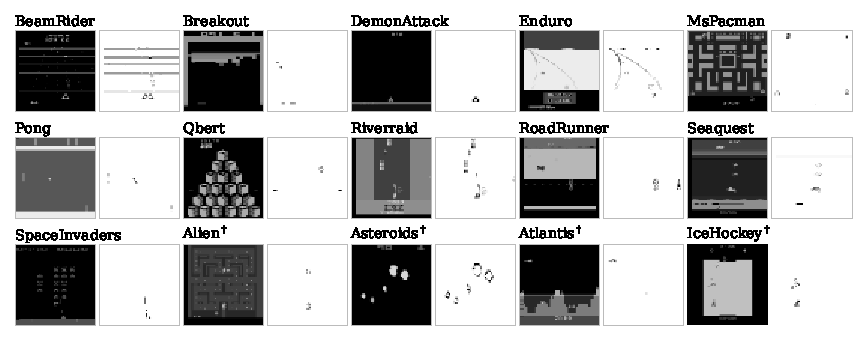
\includegraphics[width=\textwidth]{figures/games_grid.pdf}\\[0.3em]
  {\footnotesize Frame $t$ (left) and the change to the next frame (right) for all 15 games;
  $^\dagger$\,held-out games}
\end{frame}

\begin{frame}{How Different the Games Are}
  \begin{itemize}\setlength\itemsep{0.55em}
    \item \textbf{Appearance:} mean brightness 5 (DemonAttack) to 105 (Pong);
          1\% to 95\% black pixels
    \item \textbf{Motion:} in most games $<4\%$ of pixels move (Pong 1.7\%, Breakout 1.4\%)
      \begin{itemize}
        \item The important objects are a few small sprites
      \end{itemize}
    \item \textbf{Actions:} 4 to 18 actions, same index = different command per game
      \begin{itemize}
        \item Mapped to one common set of 18 ALE actions
      \end{itemize}
    \item \textbf{Episodes:} from $\sim$120 steps (Atlantis) to 12\,500 (Enduro)
    \item \textbf{Expert data:} most frequent action = 67\% of steps in RoadRunner, 99\% in
          Asteroids $\rightarrow$ few examples of alternative actions
  \end{itemize}
\end{frame}

% =================================================================
\section{Models}

\begin{frame}{Autoencoders}
  \begin{itemize}\setlength\itemsep{0.5em}
    \item \textbf{VAE:} $7\times7$ latent, too coarse for small sprites (1 epoch only)
    \item \textbf{Residual VQ-VAE:} $21\times21$ grid, codebook $K=512$, EMA updates
      \begin{itemize}
        \item Sprite-weighted version: moving pixels count $10\times$
      \end{itemize}
    \item \textbf{FSQ-VAE:} each of 4 channels rounded to $L=[8,5,5,3]$ levels
      \begin{itemize}
        \item No codebook, no commitment loss, no dead codes
        \item Resize-convolution decoder (removed checkerboard artefacts)
        \item Motion-balanced loss, moving pixels get 85\% of the weight:
      \end{itemize}
  \end{itemize}
  \[
    \mathcal{L}_{\text{bal}} = 0.85\,\tfrac{\sum m\odot(\hat x-x)^2}{\sum m}
    +0.15\,\tfrac{\sum (1-m)\odot(\hat x-x)^2}{\sum (1-m)}
  \]
  \begin{itemize}
    \item PPO feature: flattened $4\times21\times21$ grid (1\,764 values)
  \end{itemize}
\end{frame}

\begin{frame}{V-JEPA: Architecture}
  \centering
  \resizebox{\textwidth}{!}{% V-JEPA v2 architecture (atari-DQN-v2/JEPA.py), used as % V-JEPA v2 architecture (atari-DQN-v2/JEPA.py), used as % V-JEPA v2 architecture (atari-DQN-v2/JEPA.py), used as \input{figures/jepa_arch}
\resizebox{\textwidth}{!}{%
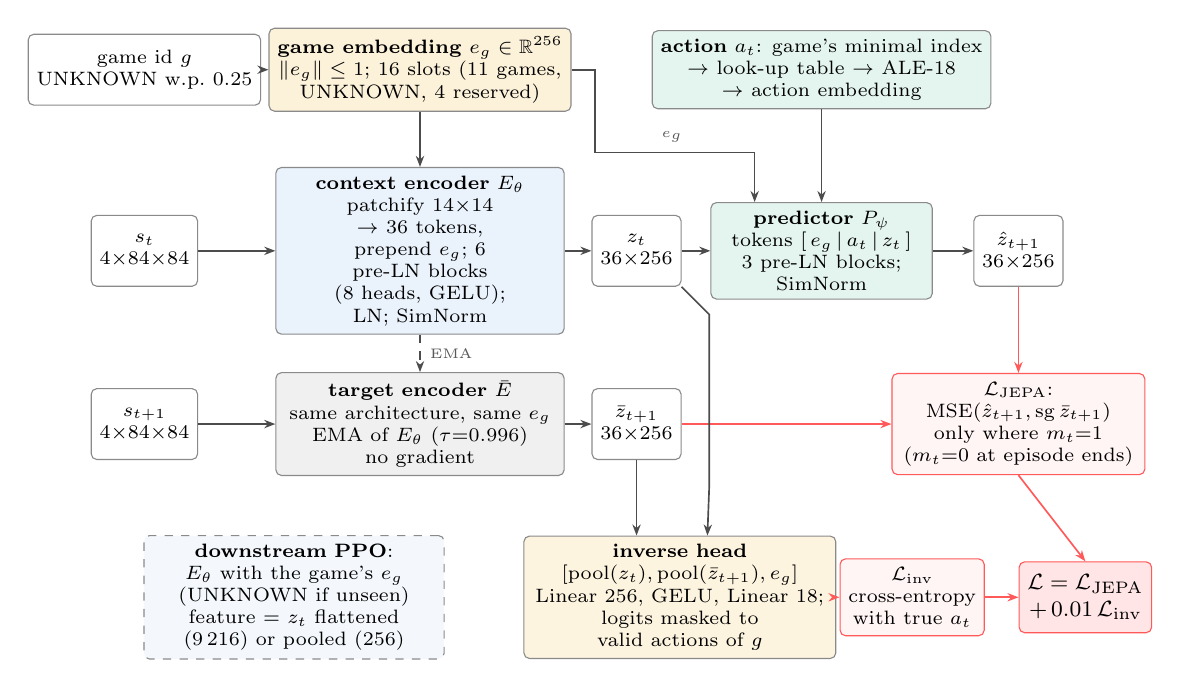
\begin{tikzpicture}[
  font=\scriptsize,
  box/.style={draw=cGray, rounded corners=2pt, align=center, inner sep=3pt, fill=white,
              minimum height=0.9cm},
  arr/.style={-{Stealth[length=4pt]}, draw=black!70, line width=0.6pt},
  larr/.style={-{Stealth[length=4pt]}, draw=red!65, line width=0.6pt},
  lab/.style={font=\tiny, text=black!65}]

  % ---------------------------------------------------------------- conditioning (top row)
  \node[box] (drop) at (0,4.5) {game id $g$\\UNKNOWN w.p.\ 0.25};
  \node[box, fill=cJep!15] (env) at (3.5,4.5)
    {\textbf{game embedding} $e_g\in\mathbb{R}^{256}$\\$\|e_g\|\le1$; 16 slots (11 games,\\UNKNOWN, 4 reserved)};
  \node[box, fill=cFsqJ!12] (act) at (8.6,4.5)
    {\textbf{action} $a_t$: game's minimal index\\$\to$ look-up table $\to$ ALE-18\\$\to$ action embedding};
  \draw[arr] (drop) -- (env);

  % ---------------------------------------------------------------- online branch
  \node[box] (st) at (0,2.2) {$s_t$\\$4{\times}84{\times}84$};
  \node[box, fill=cNat!10, text width=3.45cm] (ce) at (3.5,2.2)
    {\textbf{context encoder} $E_\theta$\\patchify $14{\times}14$ $\to$ 36 tokens,\\prepend $e_g$; 6 pre-LN blocks\\(8 heads, GELU); LN; SimNorm};
  \node[box] (zt) at (6.25,2.2) {$z_t$\\$36{\times}256$};
  \node[box, fill=cFsqJ!12, text width=2.6cm] (pr) at (8.6,2.2)
    {\textbf{predictor} $P_\psi$\\tokens $[\,e_g\,|\,a_t\,|\,z_t\,]$\\3 pre-LN blocks; SimNorm};
  \node[box] (zh) at (11.1,2.2) {$\hat z_{t+1}$\\$36{\times}256$};
  \draw[arr] (st) -- (ce); \draw[arr] (ce) -- (zt); \draw[arr] (zt) -- (pr); \draw[arr] (pr) -- (zh);
  \draw[arr] (env) -- (ce);
  \draw[arr] (act) -- (pr);
  \coordinate (ebend) at (7.75,3.45);
  \draw[arr] (env.east) -- ++(0.3,0) |- (ebend) -- (ebend |- pr.north);
  \node[lab, above] at (6.7,3.45) {$e_g$};

  % ---------------------------------------------------------------- target branch
  \node[box] (sn) at (0,0) {$s_{t+1}$\\$4{\times}84{\times}84$};
  \node[box, fill=gray!12, text width=3.45cm] (te) at (3.5,0)
    {\textbf{target encoder} $\bar E$\\same architecture, same $e_g$\\EMA of $E_\theta$ ($\tau{=}0.996$)\\no gradient};
  \node[box] (zb) at (6.25,0) {$\bar z_{t+1}$\\$36{\times}256$};
  \draw[arr] (sn) -- (te); \draw[arr] (te) -- (zb);
  \draw[arr, dashed] (ce) -- node[right, lab]{EMA} (te);

  % ---------------------------------------------------------------- losses
  \node[box, draw=red!65, fill=red!4, text width=3.0cm] (lj) at (11.1,0)
    {$\mathcal{L}_{\text{JEPA}}$: MSE$(\hat z_{t+1},\operatorname{sg}\bar z_{t+1})$\\only where $m_t{=}1$\\($m_t{=}0$ at episode ends)};
  \draw[larr] (zh) -- (lj);
  \draw[larr] (zb) -- (lj);

  \node[box, fill=cJep!12, text width=3.75cm] (inv) at (6.8,-2.2)
    {\textbf{inverse head}\\$[\operatorname{pool}(z_t),\operatorname{pool}(\bar z_{t+1}),e_g]$\\Linear 256, GELU, Linear 18;\\logits masked to valid actions of $g$};
  \draw[arr] (zt.south east) -- ++(0.35,-0.35) -- ++(0,-2.2) -- ([xshift=0.35cm]inv.north);
  \draw[arr] (zb) -- (zb |- inv.north);
  \node[box, draw=red!65, fill=red!4] (li) at (9.75,-2.2) {$\mathcal{L}_{\text{inv}}$\\cross-entropy\\with true $a_t$};
  \draw[larr] (inv) -- (li);
  \node[box, draw=red!65, fill=red!10, font=\footnotesize] (tot) at (11.95,-2.2)
    {$\mathcal{L}=\mathcal{L}_{\text{JEPA}}$\\$+\,0.01\,\mathcal{L}_{\text{inv}}$};
  \draw[larr] (li) -- (tot);
  \draw[larr] (lj.south) -- (tot.north);

  % ---------------------------------------------------------------- use in PPO
  \node[box, dashed, fill=cNat!5, text width=3.6cm] (ppo) at (1.9,-2.2)
    {\textbf{downstream PPO}: $E_\theta$ with the game's $e_g$ (UNKNOWN if unseen)\\feature = $z_t$ flattened (9\,216) or pooled (256)};
\end{tikzpicture}}

\resizebox{\textwidth}{!}{%
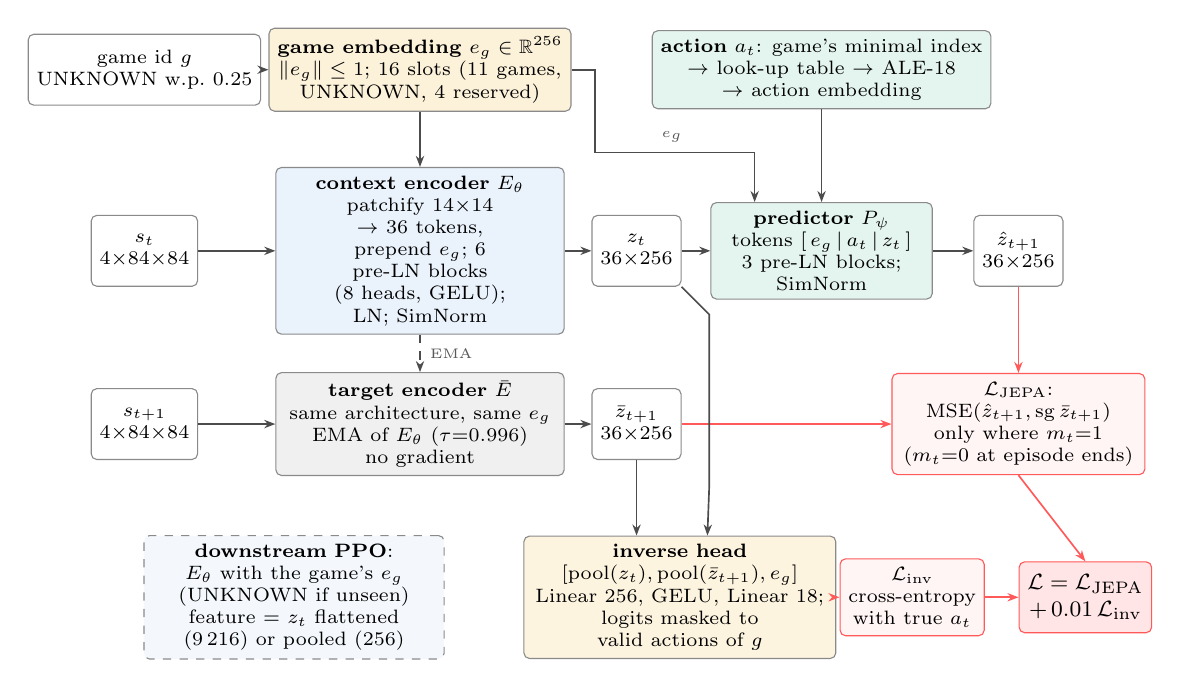
\begin{tikzpicture}[
  font=\scriptsize,
  box/.style={draw=cGray, rounded corners=2pt, align=center, inner sep=3pt, fill=white,
              minimum height=0.9cm},
  arr/.style={-{Stealth[length=4pt]}, draw=black!70, line width=0.6pt},
  larr/.style={-{Stealth[length=4pt]}, draw=red!65, line width=0.6pt},
  lab/.style={font=\tiny, text=black!65}]

  % ---------------------------------------------------------------- conditioning (top row)
  \node[box] (drop) at (0,4.5) {game id $g$\\UNKNOWN w.p.\ 0.25};
  \node[box, fill=cJep!15] (env) at (3.5,4.5)
    {\textbf{game embedding} $e_g\in\mathbb{R}^{256}$\\$\|e_g\|\le1$; 16 slots (11 games,\\UNKNOWN, 4 reserved)};
  \node[box, fill=cFsqJ!12] (act) at (8.6,4.5)
    {\textbf{action} $a_t$: game's minimal index\\$\to$ look-up table $\to$ ALE-18\\$\to$ action embedding};
  \draw[arr] (drop) -- (env);

  % ---------------------------------------------------------------- online branch
  \node[box] (st) at (0,2.2) {$s_t$\\$4{\times}84{\times}84$};
  \node[box, fill=cNat!10, text width=3.45cm] (ce) at (3.5,2.2)
    {\textbf{context encoder} $E_\theta$\\patchify $14{\times}14$ $\to$ 36 tokens,\\prepend $e_g$; 6 pre-LN blocks\\(8 heads, GELU); LN; SimNorm};
  \node[box] (zt) at (6.25,2.2) {$z_t$\\$36{\times}256$};
  \node[box, fill=cFsqJ!12, text width=2.6cm] (pr) at (8.6,2.2)
    {\textbf{predictor} $P_\psi$\\tokens $[\,e_g\,|\,a_t\,|\,z_t\,]$\\3 pre-LN blocks; SimNorm};
  \node[box] (zh) at (11.1,2.2) {$\hat z_{t+1}$\\$36{\times}256$};
  \draw[arr] (st) -- (ce); \draw[arr] (ce) -- (zt); \draw[arr] (zt) -- (pr); \draw[arr] (pr) -- (zh);
  \draw[arr] (env) -- (ce);
  \draw[arr] (act) -- (pr);
  \coordinate (ebend) at (7.75,3.45);
  \draw[arr] (env.east) -- ++(0.3,0) |- (ebend) -- (ebend |- pr.north);
  \node[lab, above] at (6.7,3.45) {$e_g$};

  % ---------------------------------------------------------------- target branch
  \node[box] (sn) at (0,0) {$s_{t+1}$\\$4{\times}84{\times}84$};
  \node[box, fill=gray!12, text width=3.45cm] (te) at (3.5,0)
    {\textbf{target encoder} $\bar E$\\same architecture, same $e_g$\\EMA of $E_\theta$ ($\tau{=}0.996$)\\no gradient};
  \node[box] (zb) at (6.25,0) {$\bar z_{t+1}$\\$36{\times}256$};
  \draw[arr] (sn) -- (te); \draw[arr] (te) -- (zb);
  \draw[arr, dashed] (ce) -- node[right, lab]{EMA} (te);

  % ---------------------------------------------------------------- losses
  \node[box, draw=red!65, fill=red!4, text width=3.0cm] (lj) at (11.1,0)
    {$\mathcal{L}_{\text{JEPA}}$: MSE$(\hat z_{t+1},\operatorname{sg}\bar z_{t+1})$\\only where $m_t{=}1$\\($m_t{=}0$ at episode ends)};
  \draw[larr] (zh) -- (lj);
  \draw[larr] (zb) -- (lj);

  \node[box, fill=cJep!12, text width=3.75cm] (inv) at (6.8,-2.2)
    {\textbf{inverse head}\\$[\operatorname{pool}(z_t),\operatorname{pool}(\bar z_{t+1}),e_g]$\\Linear 256, GELU, Linear 18;\\logits masked to valid actions of $g$};
  \draw[arr] (zt.south east) -- ++(0.35,-0.35) -- ++(0,-2.2) -- ([xshift=0.35cm]inv.north);
  \draw[arr] (zb) -- (zb |- inv.north);
  \node[box, draw=red!65, fill=red!4] (li) at (9.75,-2.2) {$\mathcal{L}_{\text{inv}}$\\cross-entropy\\with true $a_t$};
  \draw[larr] (inv) -- (li);
  \node[box, draw=red!65, fill=red!10, font=\footnotesize] (tot) at (11.95,-2.2)
    {$\mathcal{L}=\mathcal{L}_{\text{JEPA}}$\\$+\,0.01\,\mathcal{L}_{\text{inv}}$};
  \draw[larr] (li) -- (tot);
  \draw[larr] (lj.south) -- (tot.north);

  % ---------------------------------------------------------------- use in PPO
  \node[box, dashed, fill=cNat!5, text width=3.6cm] (ppo) at (1.9,-2.2)
    {\textbf{downstream PPO}: $E_\theta$ with the game's $e_g$ (UNKNOWN if unseen)\\feature = $z_t$ flattened (9\,216) or pooled (256)};
\end{tikzpicture}}

\resizebox{\textwidth}{!}{%
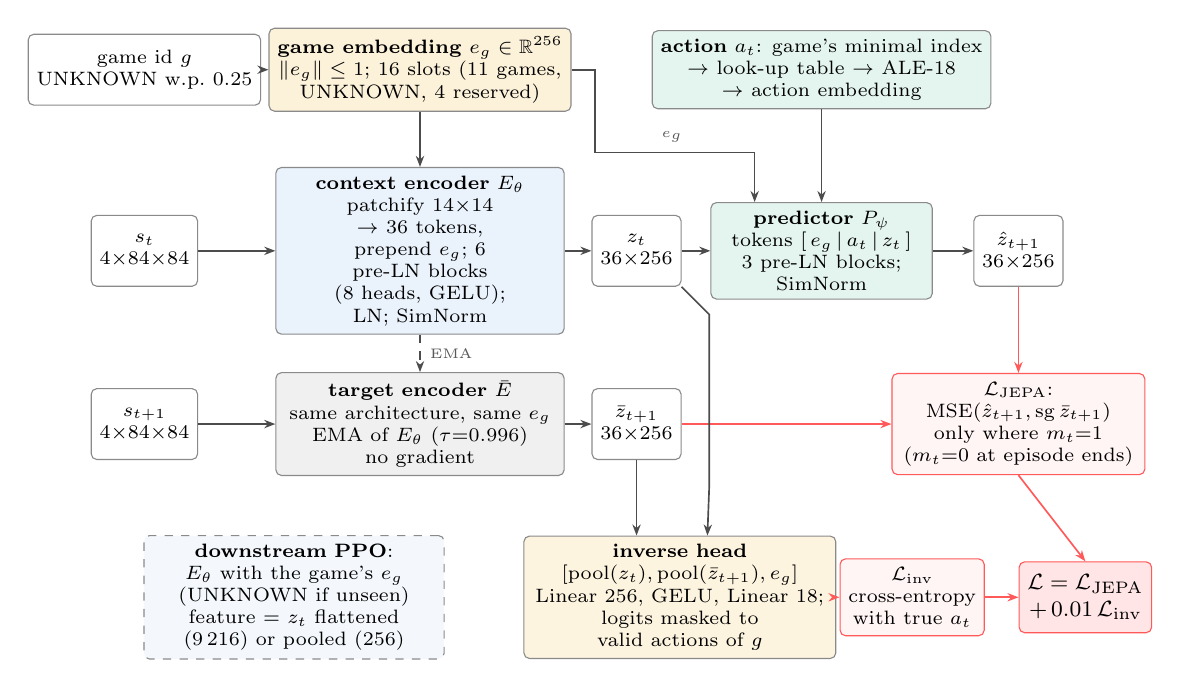
\begin{tikzpicture}[
  font=\scriptsize,
  box/.style={draw=cGray, rounded corners=2pt, align=center, inner sep=3pt, fill=white,
              minimum height=0.9cm},
  arr/.style={-{Stealth[length=4pt]}, draw=black!70, line width=0.6pt},
  larr/.style={-{Stealth[length=4pt]}, draw=red!65, line width=0.6pt},
  lab/.style={font=\tiny, text=black!65}]

  % ---------------------------------------------------------------- conditioning (top row)
  \node[box] (drop) at (0,4.5) {game id $g$\\UNKNOWN w.p.\ 0.25};
  \node[box, fill=cJep!15] (env) at (3.5,4.5)
    {\textbf{game embedding} $e_g\in\mathbb{R}^{256}$\\$\|e_g\|\le1$; 16 slots (11 games,\\UNKNOWN, 4 reserved)};
  \node[box, fill=cFsqJ!12] (act) at (8.6,4.5)
    {\textbf{action} $a_t$: game's minimal index\\$\to$ look-up table $\to$ ALE-18\\$\to$ action embedding};
  \draw[arr] (drop) -- (env);

  % ---------------------------------------------------------------- online branch
  \node[box] (st) at (0,2.2) {$s_t$\\$4{\times}84{\times}84$};
  \node[box, fill=cNat!10, text width=3.45cm] (ce) at (3.5,2.2)
    {\textbf{context encoder} $E_\theta$\\patchify $14{\times}14$ $\to$ 36 tokens,\\prepend $e_g$; 6 pre-LN blocks\\(8 heads, GELU); LN; SimNorm};
  \node[box] (zt) at (6.25,2.2) {$z_t$\\$36{\times}256$};
  \node[box, fill=cFsqJ!12, text width=2.6cm] (pr) at (8.6,2.2)
    {\textbf{predictor} $P_\psi$\\tokens $[\,e_g\,|\,a_t\,|\,z_t\,]$\\3 pre-LN blocks; SimNorm};
  \node[box] (zh) at (11.1,2.2) {$\hat z_{t+1}$\\$36{\times}256$};
  \draw[arr] (st) -- (ce); \draw[arr] (ce) -- (zt); \draw[arr] (zt) -- (pr); \draw[arr] (pr) -- (zh);
  \draw[arr] (env) -- (ce);
  \draw[arr] (act) -- (pr);
  \coordinate (ebend) at (7.75,3.45);
  \draw[arr] (env.east) -- ++(0.3,0) |- (ebend) -- (ebend |- pr.north);
  \node[lab, above] at (6.7,3.45) {$e_g$};

  % ---------------------------------------------------------------- target branch
  \node[box] (sn) at (0,0) {$s_{t+1}$\\$4{\times}84{\times}84$};
  \node[box, fill=gray!12, text width=3.45cm] (te) at (3.5,0)
    {\textbf{target encoder} $\bar E$\\same architecture, same $e_g$\\EMA of $E_\theta$ ($\tau{=}0.996$)\\no gradient};
  \node[box] (zb) at (6.25,0) {$\bar z_{t+1}$\\$36{\times}256$};
  \draw[arr] (sn) -- (te); \draw[arr] (te) -- (zb);
  \draw[arr, dashed] (ce) -- node[right, lab]{EMA} (te);

  % ---------------------------------------------------------------- losses
  \node[box, draw=red!65, fill=red!4, text width=3.0cm] (lj) at (11.1,0)
    {$\mathcal{L}_{\text{JEPA}}$: MSE$(\hat z_{t+1},\operatorname{sg}\bar z_{t+1})$\\only where $m_t{=}1$\\($m_t{=}0$ at episode ends)};
  \draw[larr] (zh) -- (lj);
  \draw[larr] (zb) -- (lj);

  \node[box, fill=cJep!12, text width=3.75cm] (inv) at (6.8,-2.2)
    {\textbf{inverse head}\\$[\operatorname{pool}(z_t),\operatorname{pool}(\bar z_{t+1}),e_g]$\\Linear 256, GELU, Linear 18;\\logits masked to valid actions of $g$};
  \draw[arr] (zt.south east) -- ++(0.35,-0.35) -- ++(0,-2.2) -- ([xshift=0.35cm]inv.north);
  \draw[arr] (zb) -- (zb |- inv.north);
  \node[box, draw=red!65, fill=red!4] (li) at (9.75,-2.2) {$\mathcal{L}_{\text{inv}}$\\cross-entropy\\with true $a_t$};
  \draw[larr] (inv) -- (li);
  \node[box, draw=red!65, fill=red!10, font=\footnotesize] (tot) at (11.95,-2.2)
    {$\mathcal{L}=\mathcal{L}_{\text{JEPA}}$\\$+\,0.01\,\mathcal{L}_{\text{inv}}$};
  \draw[larr] (li) -- (tot);
  \draw[larr] (lj.south) -- (tot.north);

  % ---------------------------------------------------------------- use in PPO
  \node[box, dashed, fill=cNat!5, text width=3.6cm] (ppo) at (1.9,-2.2)
    {\textbf{downstream PPO}: $E_\theta$ with the game's $e_g$ (UNKNOWN if unseen)\\feature = $z_t$ flattened (9\,216) or pooled (256)};
\end{tikzpicture}}
}\\[0.4em]
  {\footnotesize Predicts the \emph{latent} of the next frame stack; target encoder is an
  EMA copy (no gradients). Only the context encoder is kept for PPO.}
\end{frame}

\begin{frame}{V-JEPA: What I Changed (v1 $\rightarrow$ v2)}
  \begin{itemize}\setlength\itemsep{0.4em}
    \item v1 trained well by its loss, but a pipeline check found bugs:
      \begin{itemize}\small
        \item action indices meant different commands in different games
        \item large dataset loaded with the wrong axis order
        \item validation set contained only one game
      \end{itemize}
    \item \textbf{v2} (following TD-MPC2):
      \begin{itemize}\small
        \item common 18-action space
        \item learnable game embedding, replaced by UNKNOWN with $p=0.25$
        \item SimNorm latents ($32\times$ softmax over $V=8$) against collapse
        \item inverse-dynamics head, $\mathcal{L}=\mathcal{L}_{\text{JEPA}}+0.01\,\mathcal{L}_{\text{inv}}$
      \end{itemize}
  \end{itemize}
  \vspace{0.2em}
  {\footnotesize
  \begin{tabular}{@{}lrcc@{}}
    \toprule
    Part & Params & $\nabla\mathcal{L}_{\text{JEPA}}$ & $\nabla\mathcal{L}_{\text{inv}}$ \\
    \midrule
    Context encoder & 4.95\,M & yes & yes \\
    Predictor & 2.37\,M & yes & no \\
    Inverse head & 0.20\,M & no & yes \\
    Target encoder & 4.95\,M & \multicolumn{2}{c}{EMA only} \\
    \bottomrule
  \end{tabular}}
\end{frame}

% =================================================================
\section{Methodology}

\begin{frame}{Methodology: Pre-Training}
  \centering
  {\scriptsize\setlength{\tabcolsep}{3pt}
  \begin{tabular}{@{}lccc@{}}
    \toprule
    & Residual VQ-VAE & FSQ-VAE & V-JEPA v2 \\
    \midrule
    Data & 550\,k stacks & 550\,k stacks & 2.75\,M transitions \\
    Length & 15 epochs & 125 epochs & 92 epochs \\
    Batch & 64 & 128 & 512 \\
    Optimiser, LR & $3{\cdot}10^{-4}$ & AdamW, $3{\cdot}10^{-4}$ & AdamW, $3{\cdot}10^{-4}$ \\
    Parameters & 0.70\,M & 0.84\,M & 12.5\,M \\
    Hardware, time & Tesla T4, 3.0\,h & H100, 1.9\,h & H100, 15.6\,h \\
    \bottomrule
  \end{tabular}}
  \vspace{0.8em}
  \begin{itemize}\small\setlength\itemsep{0.4em}
    \item Architectures follow the reference papers (VQ-VAE, FSQ, I-JEPA, TD-MPC2)
    \item Smaller batch and learning rate than the JEPA papers: 12.5\,M model on one GPU
    \item V-JEPA: best validation checkpoint (epoch 90); sweep confirmed $\lambda=0.01$
  \end{itemize}
\end{frame}

\begin{frame}{Methodology: PPO and Evaluation}
  \begin{itemize}\setlength\itemsep{0.55em}
    \item \textbf{Baseline:} NatureCNN trained from scratch
    \item \textbf{Frozen:} pre-trained encoder fixed, only actor and critic trained
    \item \textbf{Fine-tuned:} pre-trained encoder trained together with the policy
    \item \textbf{PPO:} RL-Zoo Atari settings, $10$\,M steps, $8\times128$ rollouts,
          same 512-unit heads for all encoders
    \item \textbf{Metric:} mean return over steps 9--10\,M, human-normalised score
      \[\text{HNS}=\frac{\text{score}-\text{random}}{\text{human}-\text{random}}\]
    \item All numbers from the full Weights \& Biases logs, one seed per run
  \end{itemize}
\end{frame}

% =================================================================
\section{Results}

\begin{frame}{Results: Pre-Training}
  \centering
  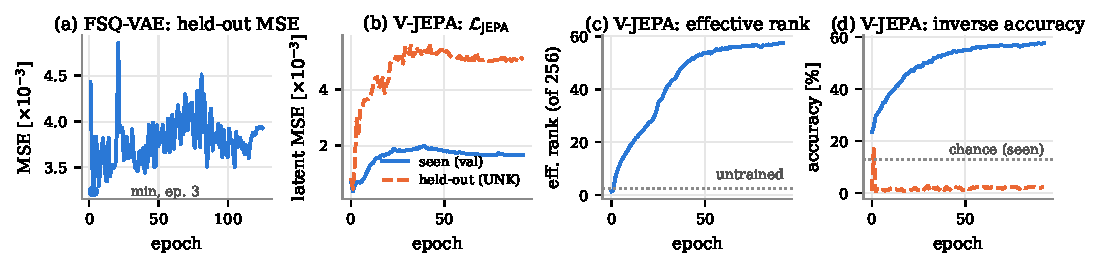
\includegraphics[width=\textwidth]{figures/pretrain_curves.pdf}
  \begin{itemize}\small\setlength\itemsep{0.35em}
    \item Held-out error is lowest \textbf{early}: FSQ-VAE best after 3 epochs, then 21\% worse
    \item V-JEPA held-out loss ends $3\times$ the seen loss $\rightarrow$ both models specialise
          to the training games
    \item V-JEPA loss \textbf{rises} while effective rank grows 1.4 $\rightarrow$ 57:
          the low early loss was a nearly collapsed latent space
    \item Reconstruction: FSQ-VAE has $3\times$ lower error on moving pixels than the VQ-VAE
  \end{itemize}
\end{frame}

\begin{frame}{Results: Downstream RL}
  \centering
  {\footnotesize\setlength{\tabcolsep}{4pt}
  \begin{tabular}{@{}lccccc@{}}
    \toprule
    & NatureCNN & \multicolumn{2}{c}{FSQ-VAE} & \multicolumn{2}{c}{V-JEPA} \\
    \cmidrule(lr){3-4}\cmidrule(lr){5-6}
    & scratch & frozen & fine-tuned & frozen & fine-tuned \\
    \midrule
    Median HNS (11 seen) & 0.74 & 0.31 & \textbf{1.07} & 0.05 & 0.04 \\
    Mean HNS (11 seen) & \textbf{2.51} & 0.54 & 2.02 & 0.13 & 0.07 \\
    Median HNS (4 held-out) & -- & 0.21 & \textbf{0.45} & -- & -- \\
    \bottomrule
  \end{tabular}}
  \vspace{0.8em}
  \begin{itemize}\small\setlength\itemsep{0.4em}
    \item \textbf{FSQ fine-tuned:} beat NatureCNN on Breakout, Enduro, Qbert, Riverraid;
          within 1\% on Pong and Seaquest
    \item NatureCNN ahead on DemonAttack, RoadRunner, BeamRider, SpaceInvaders
    \item \textbf{FSQ frozen:} learns in every game, but under a third of the fine-tuned median
    \item Fine-tuning beat freezing on 13 of 15 games (Breakout $12\times$)
    \item \textbf{V-JEPA:} learned very little in both settings
  \end{itemize}
\end{frame}

\begin{frame}{Results: Learning Curves}
  \centering
  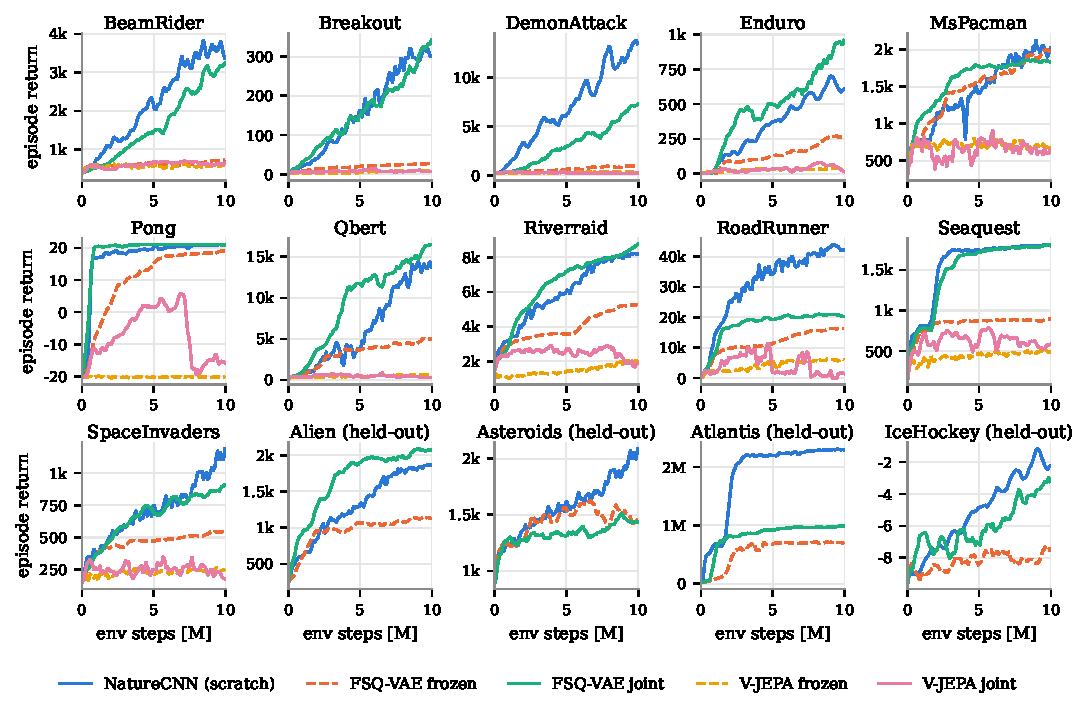
\includegraphics[width=\textwidth]{figures/learning_curves.pdf}\\[0.2em]
  {\footnotesize Solid: trained or fine-tuned encoders; dashed: frozen encoders}
\end{frame}

\begin{frame}{Results: Sample Efficiency}
  \begin{itemize}\setlength\itemsep{0.6em}
    \item Steps needed to reach 50\% / 80\% of NatureCNN's final return
    \item \textbf{FSQ fine-tuned is faster} at the 80\% level on Enduro, MsPacman, Qbert and
          Riverraid
      \begin{itemize}
        \item 1.3--2.7\,M steps earlier (18--39\%)
      \end{itemize}
    \item Faster on 5 of 11 games at the 50\% level
    \item NatureCNN is faster from the start on the games it wins
    \item Where the pre-training helps, it helps a lot
  \end{itemize}
\end{frame}

\begin{frame}{Results: Can the V-JEPA Features Be Fixed?}
  \begin{itemize}\setlength\itemsep{0.55em}
    \item First guess: the 9\,216-dim feature is too large for PPO
    \item Repeated all 22 runs with a \textbf{pooled 256-dim} feature
    \item Repeated frozen runs with a $5\times$ larger \textbf{entropy bonus}
  \end{itemize}
  \vspace{0.3em}
  \centering
  {\small
  \begin{tabular}{@{}llcc@{}}
    \toprule
    Feature & Mode & Median HNS & Critic expl.\ var. \\
    \midrule
    9\,216 (flat) & frozen & 0.045 & 0.73 \\
    256 (pooled) & frozen & 0.021 & 0.53 \\
    256 (pooled) & fine-tuned & 0.007 & $-0.27$ \\
    256, entropy 0.05 & frozen & 0.015 & 0.03 \\
    \bottomrule
  \end{tabular}}
  \vspace{0.5em}
  \begin{itemize}\small
    \item Neither change helped $\rightarrow$ the problem is \emph{what} the features encode
  \end{itemize}
\end{frame}

\begin{frame}{Results: World-Model Diagnostics}
  \begin{itemize}\setlength\itemsep{0.55em}
    \item Tested on 64 five-step sequences against a \textbf{copy baseline}, an untrained model
          and \textbf{wrong actions}
    \item \textbf{No collapse:} effective rank 52.5 vs.\ 2.5 untrained
    \item \textbf{Real dynamics:} beats copying, gap grows from $+0.013$ (1 step) to $+0.046$ (5 steps)
    \item \textbf{Weak action conditioning:} a wrong action changes the prediction by only 0.006
    \item \textbf{Game embedding unused:} encoder recognises the game from pixels
    \item \textbf{Held-out games:} worse than copying, inverse head below chance
  \end{itemize}
\end{frame}

\begin{frame}{Results: Why the V-JEPA Failed with PPO}
  \begin{columns}[T]
    \begin{column}{0.46\textwidth}
      \centering
      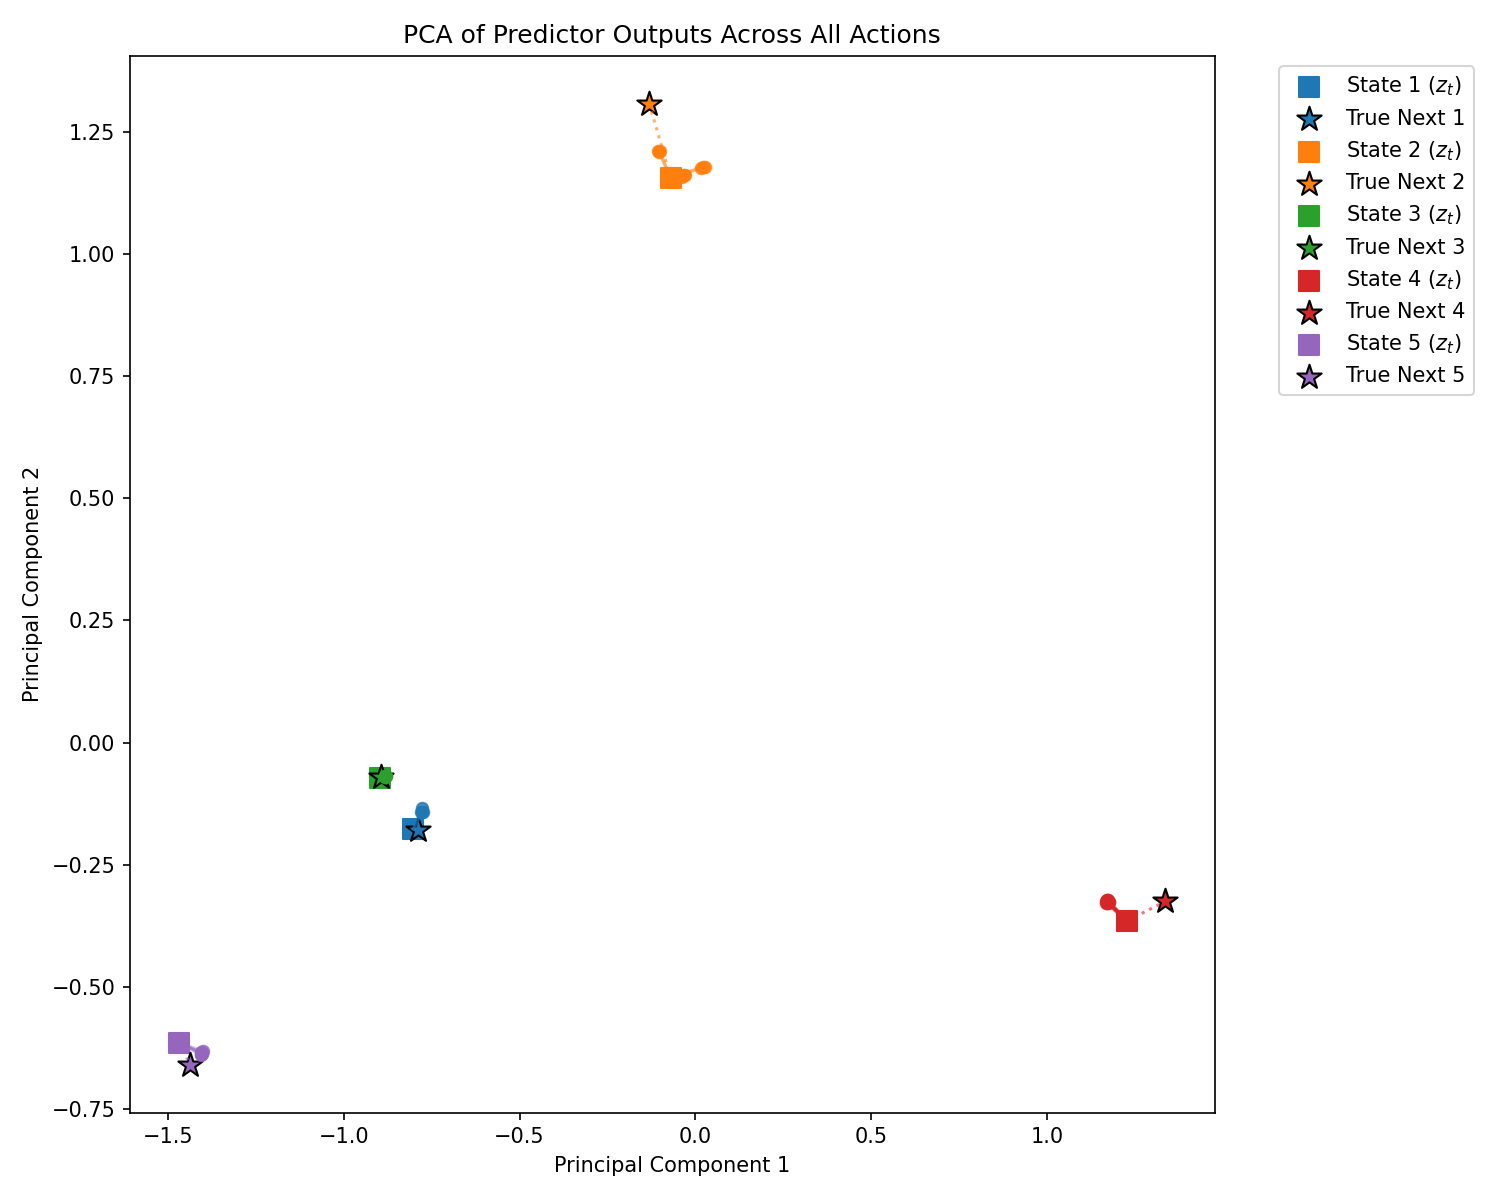
\includegraphics[width=\textwidth]{figures/pca_action_sensitivity.png}\\[0.2em]
      {\scriptsize Predictions for all actions (dots) form one tight cluster}
    \end{column}
    \begin{column}{0.54\textwidth}
      \begin{itemize}\small\setlength\itemsep{0.45em}
        \item JEPA predicts what is \emph{predictable}, small sprites can be ignored
        \item Predictor mostly ignores the action
        \item Latents change very little per step (cos.\ 0.974)
        \item $14\times14$ patches too coarse for small objects
        \item Latent space organised by game
        \item Specialised to the pre-training games
        \item Expert data shows few alternative actions
        \item Good for the \textbf{value}, not for the \textbf{best action}
      \end{itemize}
    \end{column}
  \end{columns}
\end{frame}

% =================================================================
\section{Conclusion}

\begin{frame}{Conclusion}
  \begin{itemize}\setlength\itemsep{0.55em}
    \item \textbf{RQ1:} FSQ-VAE with a motion-aware loss gave the most useful features
    \item \textbf{RQ2:} fine-tuning is clearly better than freezing
      \begin{itemize}
        \item FSQ fine-tuned is on par with NatureCNN: higher median HNS (1.07 vs.\ 0.74),
              faster learning on 4 games
      \end{itemize}
    \item \textbf{RQ3:} no model generalised to unseen games without fine-tuning
    \item \textbf{RQ4:} freezing saves little compute at this scale (976 vs.\ 854 steps/s)
    \item V-JEPA learned real dynamics, but not the \textbf{effects of actions}
    \item \textbf{Answer:} a shared encoder is a good \emph{starting point}, not yet a frozen
          replacement
  \end{itemize}
\end{frame}

\begin{frame}{Limitations and Future Work}
  \begin{itemize}\setlength\itemsep{0.55em}
    \item \textbf{Limitations:} one seed, two PPO implementations, no NatureCNN baseline on
          held-out games, PPO not re-tuned for pre-trained encoders
    \item \textbf{Future work:}
      \begin{itemize}\setlength\itemsep{0.3em}
        \item Repeat the main comparison with 3 seeds on one implementation
        \item V-JEPA with smaller patches and an action-dependent objective
              (multi-step prediction, reward head)
        \item Check features by predicting object positions before running PPO
        \item FSQ grid inside a world model, pre-training on more games
      \end{itemize}
  \end{itemize}
\end{frame}

\begin{frame}
  \vfill
  \centering
  {\Huge\bfseries Thank You!}
  \vfill
\end{frame}

\end{document}
